\documentclass{article}
\usepackage[T1]{fontenc}
\usepackage{lmodern}
\usepackage{graphicx}
\usepackage{amsmath,amssymb}
\usepackage[a4paper,margin=2cm]{geometry}
\usepackage[absolute,overlay]{textpos}
\setlength{\TPHorizModule}{1mm}
\setlength{\TPVertModule}{1mm}
\usepackage[indonesian]{babel}
\usepackage{hyperref}
\setlength{\emergencystretch}{2em}
% unit: Halaman 28

\begin{document}

% === Halaman 28 (llm) ===

\section*{3. Penyusup (\textit{intruder})}
\begin{itemize}
    \item Pihak ketiga yang menyadap, mengintersepsi, menghapus, menambah, atau mengubah pesan
    \item Sebutan lain: \textit{eavesdropper, enemy, adversary, interceptor, bad guy}, dsb
    \item Nama tokohnya: Eve, Carol, Trudy, Mallory, dsb
\end{itemize}

\vspace{40mm}

Ronald Rivest: \textcolor{red}{"cryptography is about communication in the presence of adversaries"}

% deskripsi: Diagram ilustrasi komunikasi antara Alice dan Bob yang sedang dipantau oleh Eve sebagai eavesdropper.
% bbox normalisasi: [0.2300, 0.4700, 0.7300, 0.8800]
\begin{textblock*}{105.00mm}(48.30mm,139.59mm)
\noindent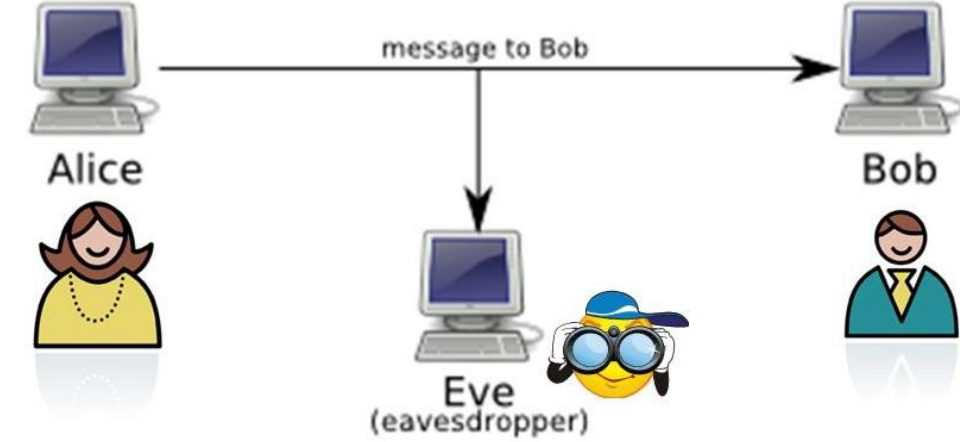
\includegraphics[width=105.00mm,height=121.77mm]{../../images/llm/page_028_img_01.png}%
\end{textblock*}

\end{document}
